\tikzset{
    leftNode/.style={circle,minimum width=.5ex, fill=none,draw},
    rightNode/.style={circle,minimum width=.5ex, fill=black,thick,draw},
    rightNodeInLine/.style={solid,circle,minimum width=.7ex, fill=black,thick,draw=white},
    leftNodeInLine/.style={solid,circle,minimum width=.7ex, fill=none,thick,draw},
  }

\section{Related Work}
\label{sec:relWork}

This chapter presents the relevant background knowledge and show approaches from other scientific paper.

\subsection{Support-Vector-Machine}

Support-Vector-Machine (SVM) is a supervised ML algorithm which classifies a set of objects (splitted in two groups) between a hyperplane in an \textit{N-dimensional} coordinate system. The goal is to find the maximum distance between the objects in both classes. As the name SVM suggest, this ML algorithm uses Support Vectors. That are the trainings data close to the hyperplane. The most maximized margin between the sets of objects is the best hyperplane. When the set of objects are more complex the SVM needs a higher dimensional hyperplane. The following example shows a two dimensional hyperplane. If linear separation is not possible a so called kernel realizes the non-linear to a feature space. The following example shows a two dimensional SVM with two classes. \\ \\

\begin{adjustbox}{center}
  \begin{tikzpicture}[
          scale=2,
          important line/.style={thick}, dashed line/.style={dashed, thin},
          every node/.style={color=black},
      ]
      \centering
      \draw[->] (-0.2,0) -- (3.5,0) node[right](xline) {};
      \draw[->] (0,-0.2) -- (0,3.5) node[right](yline) {};
      \draw[dashed line, yshift=.7cm]
         (.2,.2) coordinate (sls) -- (2.5,2.5) coordinate (sle)
         node[solid,circle,minimum width=2.8ex,fill=none,thick,draw] (name) at (2,2){}
         node[leftNodeInLine] (name) at (2,2){}
         node[solid,circle,minimum width=2.8ex,fill=none,thick,draw] (name) at (1.5,1.5){}
         node[leftNodeInLine] (name) at (1.5,1.5){}
         node [above right] {$w\cdot x + b > 1$};

      \draw[important line]
         (.7,.7) coordinate (lines) -- (3,3) coordinate (linee)
         node [above right] {$w\cdot x + b = 0$};

      \draw[dashed line, xshift=.7cm]
         (.2,.2) coordinate (ils) -- (2.5,2.5) coordinate (ile)
         node[solid,circle,minimum width=2.8ex,fill=none,thick,draw] (name) at (1.8,1.8){}
         node[rightNodeInLine] (name) at (1.8,1.8){}
         node [above right] {$w\cdot x + b < -1$};

      \draw[very thick,<->] ($(sls)+(.2,.2)$) -- ($(ils)+(.2,.2)$)
         node[sloped,above, near end] {Margin};

      \foreach \Point in {(.9,2.4), (1.3,2.5), (1.3,2.1), (2,3), (1,2.9)}{
        \draw \Point node[leftNode]{};
      }

      \foreach \Point in {(2.9,1.4), (2.3,.5), (3.3,.1), (2,0.9), (2.5,1)}{
        \draw \Point node[rightNode]{};
      }
    \end{tikzpicture}
\end{adjustbox}


\subsubsection*{Hyperplane}

The hyperplane is in a SVM a linear line between a set of objects (one set of object is called a class on one side of a hyperplane). The line differentiate the set of objects for classification. The hyperplane is used for two-dimensional coordinate systems.

\subsubsection*{Support Vector}

Support Vectors are the minimum margin on both sides of the hyperplane. The maximum margin is the nearest object to the hyperplane in both classes.

\subsubsection*{SVM optimization}

\subsubsection*{The kernel trick}

The kernel trick is used if the positions of the sets of objects is not redundant to classify them with a hyperplane. Kernel trick is also used if there are more than two classes to classify. If there
are more than two classes the SVM do a multi-class classification. The idea of multi-class classification is separating the classes in a binary classification \cite{tzotsos2008support}.

\subsection{Adversarial-Robustness-Toolbox}

For this thesis the technical framework Adversarial-Robustness-Toolbox \cite{art2018} is a main component. Nicolae et al. \cite{DBLP:journals/corr/abs-1807-01069} evaluate in their work the
technical framework ART. ART is a Python library that supports several ML frameworks for example TensorFlow and PyTorch to increase the defense of ML models. ART support 39 attacks and 29 defense'
functions. This thesis only focuses on the attack functions for poisoning attacks which will be discussed in the following section more detailed. The backdoor attacks in the technical framework
ART are introduced by Gu et al. \cite{DBLP:journals/corr/abs-1708-06733}.

\subsection{Relevant standards for risk measurement}

This present thesis based the requirements of risk measurement of ISO/IEC 27004:2009. ISO/IEC 27004:2009 - Risk Measurement is a international security standard from the ISO 27000 \cite{DBLP:conf/euspn/MeriahR19} family which guides on continious basis evaluation methods. The present ISO can be related with ISO 27001 or used as a standalone standard. In ISO 27001 it is declared as a requirement where the effectiveness must be measured of a Information Security Management System \cite{barabanov2011information}. The ISO/IEC 27004:2009 - Risk Measurement standard specifies what to be measured, when the measurement is needed and types of measurement \cite{lundholm2011design}. Barabanov et al. \cite{barabanov2011information} and Tarnes \cite{tarnes2012information} describe in their works the different properties of ISO/IEC 27004:2009 for risk measurement. Tarnes shows the information security measurement model which is shown in Figure \ref{fig:is_measurement_model}.

\begin{figure}[h!]
  \centering
  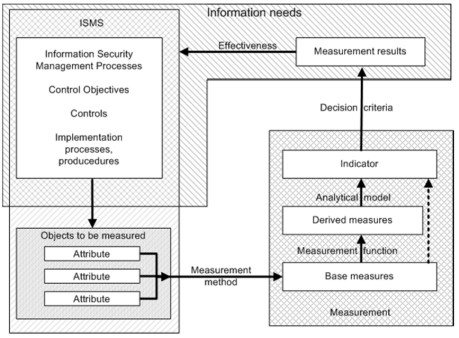
\includegraphics[width=8cm]{pictures/is_measurement_model.jpg}
  \caption{The information security measurement model \cite{tarnes2012information}}
  \label{fig:is_measurement_model}
\end{figure}

For this thesis the objects to be measured and the measurement are the important parts of the information security measurement model. The measurement method is the SMF which measure based on different properties that are derived from risk indicators that will be discussed in Subsection \ref{sec:risk_indicators}. The attributes in Figure \ref{fig:is_measurement_model} are the properties in the SMF.

\subsection{The threat model for attacker characteristics}

In their paper, Doynikova et al. \cite{DBLP:conf/crisis/DoynikovaNGK20} show a formal attacker model with input data for experiments, the data handling process and describe the experiment that was executed. Doynikova et al. explain that the attacker models can be split into high-level and low-level. These models contain attributes which used in this thesis as properties. High-level properties are subjective attributes that are obtained from monitoring the system. The gathered data are divided in three groups. The first group includes characteristics like skills, motivation and intention. The second group characterizes the attackers capabilities and show the characteristics as used resources. The last group incorporates the attacker in relation with the attacked system. This group includes the attackers location, the privileges, his goals, the access and the attackers knowledge.

\subsection{Approaches for risk measurement proposals and evaluation of risks of a ML model}
\label{sec:approaches}

This present thesis is divided into two approaches. Jakub Breier et al. \cite{DBLP:journals/corr/abs-2012-04884} propose in their paper different proposals to measure risks with different aspects.
These attacks are used in this thesis as properties to classify attacks. These different properties are attack specificity, attack time and attacker's knowledge. Attack time is split in training time
and deployment time. Training time is the attack time when the model gets manipulated while it trains. Deployment time is the attack time when the hacker attacks a ML model after its release.
Attacker's knowledge is the amount of information the hacker has available. Attackers specificity is the amount an attacker needs to manipulate the output of a ML model. These three properties may
serve as a basis for further properties useful for risk measurement. \\
Paul Schwerdtner et al. \cite{DBLP:journals/corr/abs-2011-04328} is the second approach of this thesis. Schwerdtner et al. show a technical framework to evaluate the risks for ML models. Schwerdtner et
al. give an evaluation whether it is secure to deploy a ML model or not. The ML model in Schwerdtner et al. must be a fully developed ML model that is trained and tested. Schwerdtner et al. concentrate
on inference data when the ML model is executed. This thesis discuss this paper as an approach to estimate where the RMF could be used for.

\subsection{Security risks in context of Machine Learning}

Security risks in context of ML must be derived from classic IT security risks in context to classic applications.
Xiao et al. \cite{DBLP:conf/sp/XiaoLZX18} evaluate the security risks in deep learning for common frameworks, for example TensorFlow. Xiao et al. uses the framework sample applications along the
frameworks. One statement of Xiao et. al is that the named frameworks TensorFlow, Caffe and Torch are implemented with many lines of code which make them vulnerable for many security vulnerabilities
for example heap overflow or integer overflow. Xiao et. al work is only in context of deep learning e.g. only for neural networks.

\subsubsection*{Backdoor Attacks}
\label{sec:backdoor}
Due to the rising amount of training data, human supervision to check trustworthiness is less possible. That exposes vulnerabilites in training datasets like backdoors. Backdoor attacks can cause far-
reaching consequences for example bypass critical authentication. In \cite{DBLP:journals/corr/abs-2003-03675} Salem et al. introduces dynamic backdoors to trigger (a secret pattern of neighboring
pixels) random patterns and locations to reduce the efficacy on identifying backdoors. Salem et al. discuss in their work three backdoors, Random Backdoor, Backdoor Generating Network and Conditional
Backdoor Generating Network.
Gu et al. show in their paper different backdoor attacks and do a case study with a traffic sign detection attack. The evaluated backdoors are a single pixel backdoor and a pattern backdoor. The single
pixel backdoor increase the brightness of a pixel and the pattern backdoor adds a pattern of bright pixels in an image. The implemented attacks from Gu et al. are single target attack and an all-to-all attack.

\subsection{Risk assessment in context of Machine Learning}

Risk assessment in context of ML is derived from classic IT security risk assessment. This subsection discusses paper from classic IT security risk assessment and abstract them to ML. Sendi et al. \cite{DBLP:journals/compsec/SendiAC16} evaluates the taxonomy of risk assessment and at which point in IT security management risk measurement takes place for the thesis and how it is carried out. In their paper, Sendi et al. evaluated 125 works published between 1995 and 2014. They developed categories for risk analysis which are appraisementn perspective, resource valuation and the last category is risk measurement. This category is the last step of risk assessment. To evaluate risks by measuring them, there are different properties which have an impact for risk measurement. Sendi et al. explain that the type of the attack, the dependency severity between resources and the type of defined permissions between resources are needed to measure risks. Risk measurement in their paper is differentiated between non-propagated and propagated. Non-propagated risk measurement stands in relation to the resource valuation category leading to the example of business driven risk assessment. Business driven is the view of business oriented goals and processes. And non-propagated risk measurement means that a model in which the risks are measured without the impact from other resources. For example, if the risks are measured business driven, the parameters such as business process are seen without the impact from other business processes. Propagated risk measurement concentrates on the attack impact and its propagation on other resources. The risk measurement is measuring the propagated risks as a dependency graph. That means an compromised parent node could propagate connected nodes backwards and forward. Backward impact means the impact propagation on all nodes that have a dependency with the compromised node and forward impact is the propagation from the compromised node to all its dependent nodes. In context to ML the propagated risk measurement is important because for example in context of this thesis a manipulated trainings and testing dataset could lead a more extent missclassification while training and testing.
